\chapter{Implementation and Experiments} \label{chp:experiments}

\section{Experimental Setup}
All experiments were conducted on a consistent hardware and software platform to ensure fair and reproducible comparisons. This section details the environment and datasets used in our evaluation.

\subsection{Hardware}
The experimental platform is a MacBook Pro equipped with an Apple M4 Pro processor and 24 GB of RAM, running macOS. 

\begin{comment}
In brief, paper ~\cite{kolmogorovBlossomNewImplementation2009} presents Blossom~V, a practical implementation of Edmonds’ blossom algorithm for computing minimum-cost perfect matchings in undirected weighted graphs. While the theoretical worst-case bounds for the blossom family have steadily improved since Edmonds’ original $O(n^2m)$ algorithm, Blossom~V is designed for strong empirical performance rather than new asymptotic guarantees. It combines two ingredients that had proven effective separately in prior work: the variable $\delta$ (variable dual updates) strategy popularized by Blossom~IV, and systematic use of priority queues to efficiently select minimum-slack edges.

Blossom~V targets general (not necessarily bipartite) graphs, and thus directly applies to our bipartite instances as a special case. In our experiments we use the publicly available Blossom~V implementation as a black-box solver to compute minimum-cost perfect matchings for the graphs generated by our compression pipeline.
\end{comment}

\subsection{Datasets}
To systematically evaluate performance under controlled conditions, particularly with respect to repetitiveness, we generated a suite of synthetic labeled tries. Real-world datasets often lack ground-truth information about their repetitive structures, making it difficult to isolate the effects of this property. Our synthetic generation approach allows us to create trees with tunable characteristics.

The tries were generated using a custom Python script that constructs a tree and introduces repetitiveness by randomly copying subtries to different locations. At each step of the tree's growth, with a certain probability, a random existing subtrie is selected and duplicated as a new branch. This ``copy-paste'' mechanism allows us to create complex, highly repetitive structures that mimic patterns found in real-world data.

The generation process was controlled by the following key parameters:
\begin{description}
    \item[Max Branching Factor] The maximum number of children for any node.
    \item[Repetition Probability] The probability of copying an existing subtrie instead of creating a new random branch.
    \item[Subtrie Depth Range] The minimum and maximum depth of subtries eligible for copying.
    \item[Max Nodes] The target maximum number of nodes in the generated trie.
    \item[Alphabet Size] The number of unique characters in the alphabet.
    \item[Seed] The seed used for random number generation to ensure reproducibility.
\end{description}

By varying these parameters, we can produce a diverse range of tries to thoroughly test the limits and behaviors of each compression algorithm.

\section{XBWT Implementation and Experiments}
Before presenting the implementation and the experiments related to our proposed trie compression scheme, it is necessary to detail our implementation of the XBWT introduced in \cref{sec:XBWT}. This implementation serves a dual purpose. Firstly, it provides the \textsc{PathSort} algorithm, a fundamental component required by our compression method. Secondly, it will serve as a benchmark for comparison against our scheme in future work. For now, our focus is on the experiments conducted to evaluate the performance of the \textsc{PathSort} algorithm, particularly its execution time.

\section{Implementation}
The XBWT data structure has been implemented in C++ using the Succinct Data Structure Library 2.0 (SDSL) for efficient representation and manipulation of compressed data structures. We will develop two algorithms for constructing the XBWT: one efficient linear-time recursive algorithm and one more straightforward iterative algorithm. Also, we will implement the necessary data structures and algorithms for navigating and querying the XBWT, such as parent-child navigation and path-based searches. 

The implementation of the XBWT is based on the descriptions provided in the previous sections. Also, it is available on GitHub at the following link: \url{https://github.com/davide-tonetto-884585/XBWT}.

\subsection{Implementation Choices}
Follows a list of the main choices made during the implementation of the XBWT:
\begin{itemize}
    \item The implementation is not focused on a specific kind of data, such as XML documents or JSON files, but it is designed to work with any kind of labeled tree. 
    \item The construction method takes as input a labeled tree. It constructs directly a compressed indexing scheme based on the Extended Burrows-Wheeler Transform of the tree as described in the previous sections.
    \item For the XBWT to work, we assume that the labels of the leaf nodes of the given labeled tree are lexicographically greater than the labels of the internal nodes. This is necessary to ensure that the navigational and search operations work correctly. \draft{This can be obtained by...} \alessio{spiega come si ottiene questo risultato nel caso le foglie siano più piccole.}
    \item The implementation is based on the Succinct Data Structure Library (SDSL) to handle the compressed data structures generated by the XBWT. The SDSL library provides efficient implementations of various compressed data structures and algorithms, which are essential for representing and querying the XBWT efficiently.
    \item The labels of the alphabet are encoded as integers, starting from 0 to $|\Sigma| - 1$, where $|\Sigma|$ is the cardinality of the alphabet. This encoding respects the order of the labels in the alphabet and allows simplifying and reducing the space needed to store the labels in the compressed data structure. For this reason, the constructor of the XBWT class takes as input a generic labeled tree.
    \item All the operations introduced in \cref{sec:xbwt_operations} are implemented in the XBWT class.
\end{itemize}

\subsection{Succinct Data Structures}
The implementation of the XBWT relies heavily on succinct data structures to achieve space efficiency while maintaining fast query operations. In particular, we use succinct data structures to compress the two main arrays of the XBWT: $S_\alpha$ and $S_{\text{last}}$. These arrays, which can be quite large for substantial trees, benefit significantly from compression.

The compression is achieved through the Succinct Data Structure Library (SDSL), which provides efficient implementations of various compressed data structures. For $S_{\text{last}}$, which is a binary sequence, we utilize a compressed bit vector that supports fast rank and select operations. For $S_\alpha$, which contains labels from a potentially large alphabet, we employ a wavelet tree structure that provides both compression and efficient query capabilities.

The SDSL is a C++ library that provides efficient implementations of various compressed data structures and algorithms. It is used in this project to handle the compressed data structures generated by the XBWT. The SDSL library provides a wide range of succinct data structures, such as bit vectors, wavelet trees, and compressed suffix arrays, which are essential for representing and querying the XBWT efficiently. The library is available at \url{https://github.com/simongog/sdsl-lite} \cite{gbmp2014sea}. Let's see the implementation details of the SDSL data structures used in the XBWT implementation.

\subsubsection{RRR Bit Vector}
The RRR bit vector is designed to provide space-efficient representations of bit vectors while supporting efficient rank and select operations. This data structure implements the RRR (Raman, Raman, and Rao) encoding method, which compresses bit vectors by partitioning them into fixed-size blocks and encoding each block based on its population count (the number of 1s) and specific configuration \cite{raman2002succinct}. 

The space needed for an RRR bit vector of length $n$ with $m$ set bits is $nH_0 + o(n)$ ($\approx \lceil \log \binom{n}{m} \rceil$). 
The rank support is provided by \texttt{sdsl::rank\_support\_rrr}, adding $80$ bits and requiring $O(\log k)$ time for rank queries, where $k$ is the number of set bits. The select support is provided by \texttt{sdsl::select\_support\_rrr}, adding $64$ bits and requiring $O(\log n)$ time for select queries.

This data structure is used to represent the $S_{\text{last}}$, the additional bit in $S_{\alpha}$, and $A$ arrays of the XBWT.

\subsubsection{Wavelet Tree}
The Wavelet tree is designed to efficiently handle sequences over large alphabets, such as integer sequences. It provides a space-efficient representation while supporting fast access, rank, and select operations. The wavelet tree is a balanced binary tree that recursively partitions the alphabet into two equal-sized subsets and encodes the sequence based on the partitioning \cite{grossi2003high}. The \texttt{sdsl::wt\_int} uses the RRR bit vectors or other succinct representations for storing the bit vectors in each node of the wavelet tree. This makes the structure space-efficient.

In the case of RRR bit vectors the space needed by integer Wavelet tree for a sequence of length $n$ over an alphabet of size $\sigma$ is $nH_0(S) + o(n \log \sigma) + \Theta(\sigma \log n)$ bits, where $H_0(S)$ is the zero-order empirical entropy of the sequence $S$. Also supports query access, rank, and select operations in $O(\log \sigma)$ time.

This data structure is used to represent the $S_\alpha$ array of the XBWT.

\begin{comment}
\subsection{Details of the XBWT Class Elements}
\alessio{Questa sezione non mi convince. Non descrivere troppo il codice, la documentazione dovrebbe essere nella repo e nel codice, non nella tesi.}
The XBWT class utilizes several data structures from the SDSL library to efficiently represent and query the compressed data. Below are the details of the main elements used in the class:

\begin{itemize}
    \item \texttt{sdsl::rrr\_vector<> SLastCompressed}: This is a compressed bit vector that stores the $S_{\text{last}}$ array of the XBWT. 
    \item \texttt{sdsl::wt\_int<sdsl::rrr\_vector<>> SAlphaCompressed}: This is a wavelet tree built on top of a compressed bit vector. The wavelet tree is used to compress and index the $S_{\alpha}$ array of the XBWT.
    \item \texttt{sdsl::rrr\_vector<> SAlphaBitCompressed}: Another compressed bit vector used to store the additional bit of $S_{\alpha}$ needed to distinguish between internal and leaf nodes.
    \item \texttt{sdsl::rrr\_vector<> ACompressed}: A compressed bit vector representing the $A$ array of the XBWT used to in the $F$ array of the XBWT.
    \item \texttt{sdsl::rrr\_vector<>::rank\_1\_type SLastCompressedRank}: A rank support structure for the \texttt{SLastCompressed} bit vector, allowing efficient rank queries.
    \item \texttt{sdsl::rrr\_vector<>::select\_1\_type SLastCompressedSelect}: A select support structure for the \texttt{SLastCompressed} bit vector, allowing efficient select queries.
    \item \texttt{sdsl::rrr\_vector<>::rank\_1\_type ACompressedRank}: A rank support structure for the \texttt{ACompressed} bit vector.
    \item \texttt{sdsl::rrr\_vector<>::select\_1\_type ACompressedSelect}: A select support structure for the \texttt{ACompressed} bit vector.
    \item \texttt{std::unordered\_map<T, unsigned int> alphabetMap}: A hash map that maps each label in the alphabet to a unique integer.
    \item \texttt{unsigned int cardSigma}: The cardinality of the alphabet $\Sigma$.
    \item \texttt{unsigned int cardSigmaN}: The cardinality of the $\Sigma_N$ alphabet. Where $\Sigma_N$ is the set of labels that appear in the internal nodes of the labeled tree.
    \item \texttt{unsigned int maxNumDigits}: The maximum number of digits that has the integer code associated to the greater label in the alphabet (needed to sort the labels in the alphabet).
\end{itemize}

The overall space complexity of the XBWT class can be derived from the space complexity of the compressed data structures used in the class. 

\subsection{Construction implementation}
\alessio{Perché non fare pseudocodice come per Alg 1?}
The construction of the XBWT is done by the constructor of the XBWT class. The constructor takes as input a generic labeled tree and constructs the compressed indexing scheme using the linear pathSort (also the naive construction method can be used by passing the boolean flag \texttt{usePathSort = false}). The construction process is divided into the following steps:

\begin{enumerate}
    \item \textbf{Alphabet Encoding}: The first step is to encode the labels of the alphabet as integers. The labels are sorted in lexicographical order and assigned a unique integer code starting from 1 to $|\Sigma|$. Two hash maps are used to map each label to a unique integer and vice versa. 
    \item \textbf{Construct \texttt{intNodes} array}: The next step is to construct the \texttt{intNodes} array as described in the previous chapters. \texttt{intNodes} is an array of triplets of length $t$ in which node is represented as a triplet containing the node's label, its level, and the index of its parent node in the array (from 1 to t, root has parent 0). The nodes are inserted in preorder traversal of the labeled tree.
    \item \textbf{Sort \texttt{intNodes} array:} Call the \texttt{pathSort} or \texttt{upwardStableSortConstruction} (naive method) method to get the sorted array of nodes \texttt{intNodes}.
    \item \textbf{Construct $S_{\text{last}}$ array}: Construct the $S_{\text{last}}$ array by iterating over the sorted \texttt{intNodes} array.
    \item \textbf{Construct $S_{\alpha}$ array}: Construct the $S_{\alpha}$ array by iterating over the sorted \texttt{intNodes} array, along with the additional bit array to distinguish between internal and leaf nodes.
    \item \textbf{Construct $A$ array}: Construct the $A$ array by iterating over the sorted \texttt{intNodes} array.
    \item \textbf{Construct rank and select support structures}: Construct the rank and select support structures for the compressed bit vectors.
\end{enumerate}

\subsection{Navigational Operations}
\alessio{Non basta dire che implementi tutte le funzioni descritte nella sezione 3.7?}

The XBWT class provides several navigational operations to traverse the labeled tree and retrieve information about the nodes. The navigational operations implemented are:

\begin{itemize}
    \item \texttt{getChildren(unsigned int i)}: This method returns a pair of integers representing the indices of the leftmost and rightmost children of the node at index \texttt{i}.
    \item \texttt{getRankedChild(unsigned int i, unsigned int k)}: This method returns the index of the \texttt{k}-th child of the node at index \texttt{i}.
    \item \texttt{getCharRankedChild(unsigned int i, T label, unsigned int k) const}: This method returns the index of the \texttt{k}-th child of the node at index \texttt{i} with the specified label.
    \item \texttt{getDegree(unsigned int i)}: This method returns the degree (number of children) of the node at index \texttt{i}.
    \item \texttt{getCharDegree(unsigned int i, T label)}: This method returns the number of children of the node at index \texttt{i} with the specified label.
    \item \texttt{getParent(unsigned int i)}: This method returns the index of the parent of the node at index \texttt{i}.
    \item \texttt{getSubtree(unsigned int i, unsigned int order = 0)}: This method returns a vector containing the labels of the nodes in the subtree rooted at index \texttt{i}. The \texttt{order} parameter specifies the traversal order (e.g., preorder, post-order).
\end{itemize}

All the methods refer to the index of the nodes in $S_{\text{last}}$ and $S_{\alpha}$ arrays. 

\subsection{Search Operations}
The XBWT class provides search operation \texttt{subPathSearch(const std::vector<T> \&path)} that searches for a subpath in the XBWT structure. It uses the compressed vectors to determine the range of positions corresponding to the nodes whose upward path is prefixed by a given vector reversed.

\end{comment}

\subsection{Construction Time Experiments} 

To evaluate the performance of the implemented algorithms, we conducted a series of experiments on randomly generated trees, with sizes ranging from 100 to 900,000 nodes. For each tree, we executed the construction algorithms 10 times, recording the average execution time for both the linear \textsc{PathSort} algorithm and the Naive Sort algorithm used for constructing the XBWT.
By ``Naive Sort'', we refer to a straightforward approach that first precomputes all the upward paths in the tree and then sorts them using a standard sorting algorithm. This method contrasts with \textsc{PathSort}, which is specifically designed to achieve linear time complexity in path sorting.
This approach enabled us to compare their performance across various tree sizes and evaluate their scalability.

From the results shown in Table \cref{tab:experiments}, we can draw several conclusions about the performance of the \textsc{PathSort} algorithm compared to the Naive Sort algorithm.

The \textsc{PathSort} algorithm consistently outperforms the Naive Sort algorithm in terms of execution time, especially as the number of nodes increases. For smaller trees, the difference in execution time between the two algorithms is minimal. However, as the number of nodes grows, the \textsc{PathSort} algorithm demonstrates significantly better scalability. For instance, with 900,000 nodes, the \textsc{PathSort} algorithm takes 8.51 seconds, whereas the Naive Sort algorithm takes 34.2 seconds, giving a speedup of more than $4\times$. A visual representation of the results can be seen in \cref{fig:xbwt_exp_plots} where both the time comparison and the speedup are shown.

\begin{table}[h]
    \centering
    \begin{tabular}{|r|r||r|r|}
        \hline
        \textbf{\# Nodes} & \textbf{Depth} & \textbf{Naive Sort (s)} & \textbf{\textsc{PathSort} (s)} \\
        \hline
            100 &    22 &  0.001 & 0.002 \\
            500 &    45 &  0.002 & 0.004 \\
          1,000 &    74 &  0.003 & 0.006 \\
          5,000 &   175 &  0.015 & 0.028 \\
         10,000 &   288 &  0.053 & 0.056 \\
         50,000 &   486 &  0.350 & 0.310 \\
        100,000 &   754 &  1.250 & 0.690 \\
        500,000 & 2,246 & 16.460 & 4.700 \\
        900,000 & 2,658 & 34.200 & 8.510 \\
        \hline
    \end{tabular}
    \caption{Performance comparison of the execution times for the Naive Sort and \textsc{PathSort} algorithms on randomly generated trees of varying sizes.}
    \label{tab:experiments}
\end{table}

\begin{figure}[H]
    \centering
    \begin{subfigure}[b]{0.48\textwidth}
        \centering
        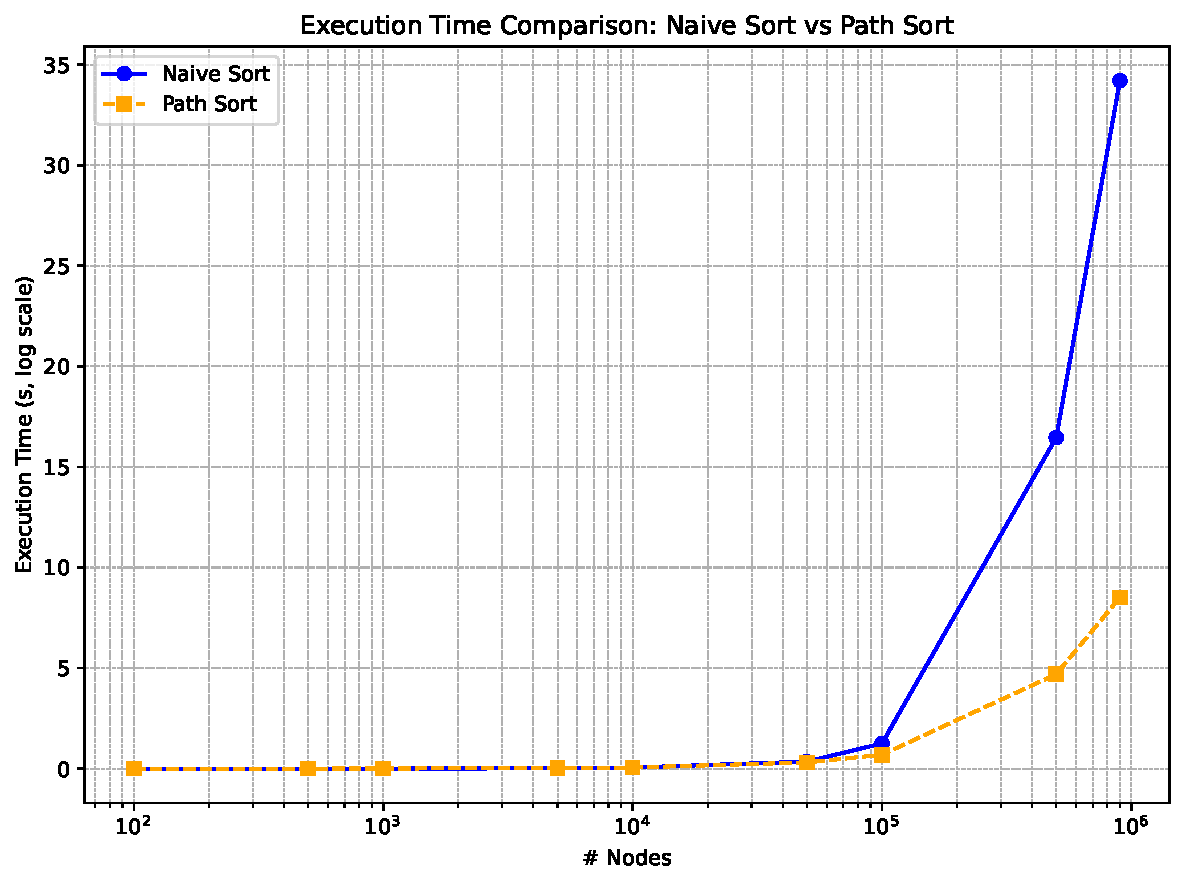
\includegraphics[width=\textwidth]{"Immagini/execution_time_comparison.pdf"}
        \caption{Time Comparison}
        \label{fig:time_comparison}
    \end{subfigure}
    \hfill %
    \begin{subfigure}[b]{0.48\textwidth}
        \centering
        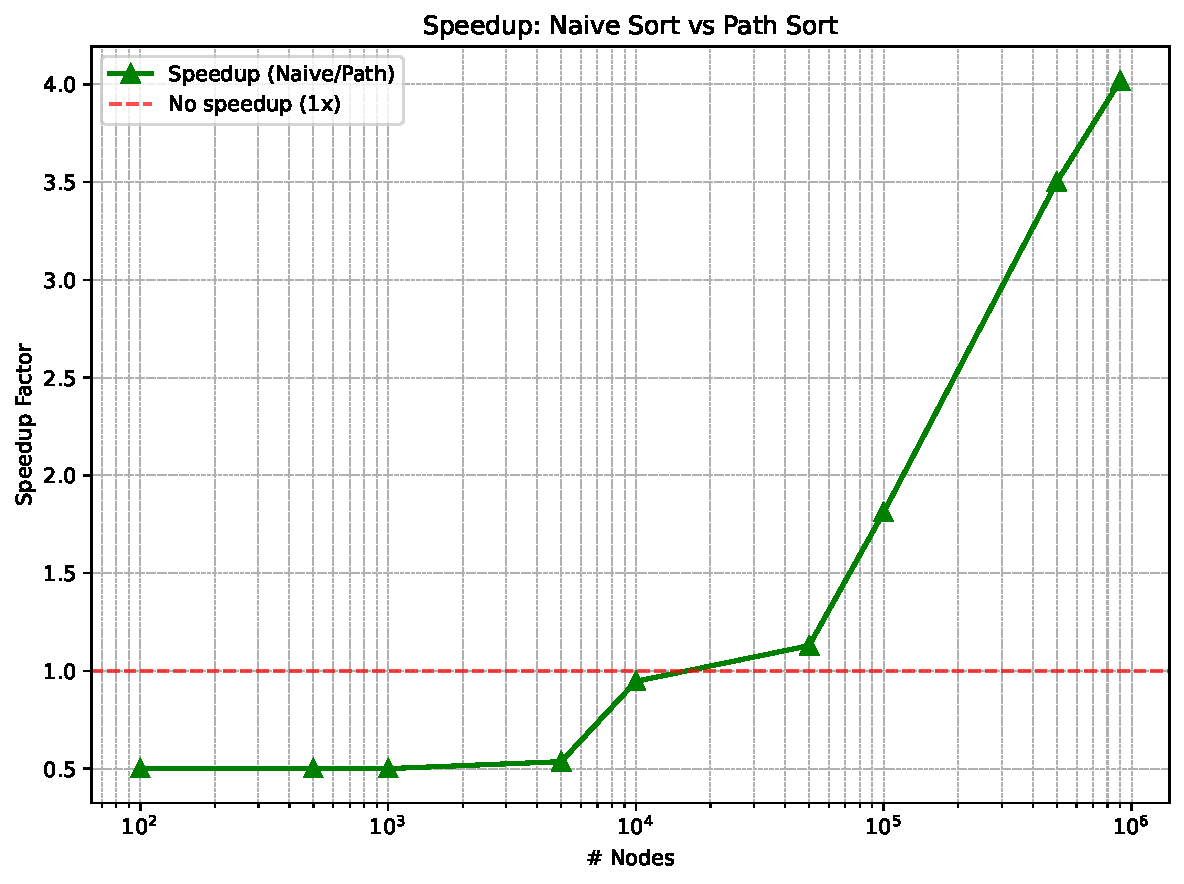
\includegraphics[width=\textwidth]{"Immagini/speedup_comparison.pdf"}
        \caption{Speedup}
        \label{fig:speedup}
    \end{subfigure}
    \caption{Time comparison and speedup plots for the experiments in \cref{tab:experiments}. Image (a) shows \textsc{PathSort} time in seconds (yellow dashed line) vs. Naive Sort time (blue line). Image (b) shows the speedup of \textsc{PathSort} over Naive Sort. The area below the red dashed line indicates points where the speedup is less than or equal to 1, representing no improvement of \textsc{PathSort} over Naive Sort.}
    \label{fig:xbwt_exp_plots}
\end{figure}

\begin{comment}
\subsubsection{Space Analysis}
To evaluate the space savings achieved through XBWT compression, we conducted experiments on the same set of randomly generated trees used for the construction performance tests. For each tree, we compared the memory usage (in bytes) of three representations: the plain tree, the uncompressed XBWT, and the compressed XBWT.

The plain tree representation consists of the simple balanced parentheses encoding of the tree structure combined with the edge labels. For example, for the tree in \cref{fig:example_tree,tab:xbwt_example}, the plain tree representation would be:

\texttt{(A(B(D(a))(a)(E(b)))(C(D(c))(b)(D(c)))(B(D(b))))}.

By \emph{uncompressed XBWT}, we refer to the XBWT arrays $S_{\text{last}}$ and $S_{\alpha}$ (including the additional bit) stored without any compression. Specifically, $S_{\text{last}}$ is represented as a plain bitvector (\texttt{sdsl::bit\_vector}), and $S_{\alpha}$ is stored as a wavelet tree (\texttt{sdsl::wt\_int}) with plain bitvectors (\texttt{sdsl::bit\_vector}). In contrast, the \emph{compressed XBWT} representation stores $S_{\text{last}}$ and $S_{A}$ as compressed RRR bitvectors (\texttt{sdsl::rrr\_vector}), and $S_{\alpha}$ as a wavelet tree with RRR bitvectors, as described in the previous chapter.

\cref{tab:experiments_2} reports the sizes (in bytes) for each representation of the trees across different sizes. The last column highlights the space savings achieved by the compressed XBWT compared to the plain tree representation, expressed as a percentage. These results illustrate the substantial space reductions achieved through compression, especially as the tree size increases.

%\alessio{Oltre ai punti di prima, metti la percentuale anche per UXBWT, magari non come un'altra colonna ma metti tra parentesi. Te lo faccio sulle prime righe per la C.XBWT. Se ti piace, ricorda di spiegare cosa sono i numeri tra parentesi nella descrizione.}
\begin{table}[ht]
    \centering
    \begin{tabular}{|r||r|r|r|}
        \hline
        \textbf{\# Nodes} & \textbf{Plain tree} & \textbf{U. XBWT} & \textbf{C. XBWT} \\
        \hline
            100 &       390 &       424 &       496 \color{gray}{(-27.18\%)}\\
            500 &     2,390 &     1,112 &     1,136 ~\color{gray}{(52.47\%)} \\
          1,000 &     4,890 &     2,242 &     2,056 ~\color{gray}{(57.96\%)} \\
          5,000 &    28,890 &    12,911 &    10,400 ~\color{gray}{(64.00\%)} \\
         10,000 &    58,890 &    45,625 &    21,848 ~\color{gray}{(62.90\%)} \\
         50,000 &   338,890 &   175,146 &   123,216 ~\color{gray}{(63.64\%)} \\
        100,000 &   688,890 &   349,478 &   259,376 ~\color{gray}{(62.35\%)} \\
        500,000 & 3,888,890 & 1,850,850 & 1,451,570 ~\color{gray}{(62.67\%)} \\
        900,000 & 7,088,890 & 3,480,190 & 2,718,570 ~\color{gray}{(61.65\%)} \\
        \hline
    \end{tabular}
    \caption{Space analysis of the XBWT. The first column represents the number of nodes, the others the bytes used by each representation.
    ``Plain tree'' is the size of the tree in the simple balanced parenthesis representation plus the edge labels, ``U. XBWT'' is the size of the uncompressed XBWT, and ``C. XBWT'' is the size of the compressed XBWT.
    Gray numbers between parentheses represent the improvement relative to the plain tree representation.}
    \label{tab:experiments_2}
\end{table}

For small trees, the compressed XBWT does not always provide immediate savings due to the overhead of succinct data structures. For instance, for 100 nodes, the compressed representation is larger than the plain tree, showing a \(-27.18\%\) increase in space. However, as the number of nodes increases, the compression becomes more effective, achieving savings of over 60\% for large trees.

The space reduction becomes particularly evident for trees with more than 500 nodes. These results confirm that the compressed XBWT provides a scalable and space-efficient alternative for storing and indexing labeled trees. The efficiency gains are particularly beneficial for applications requiring large-scale tree processing, such as bioinformatics and text indexing.
\end{comment}


\section{Trie Compression Scheme Implementation and Experiments}

\subsection{Implementation}
Our proposed trie compression scheme was implemented in C++ to run some preliminary experiments and it is available at \url{https://github.com/davide-tonetto-884585/trie-compression}. We compiled it using Apple Clang 17. 

In particular, we utilized the \textsc{PathSort} algorithm implementation of the XBWT introduced in \cref{sec:xbwt_impl}. Moreover, we used a C++ implementation by Vladimir Kolmogorov of the minimum cost perfect matching algorithm described in~\cite{kolmogorovBlossomNewImplementation2009}. The implementation is available at \url{https://pub.ista.ac.at/~vnk/software.html}.

\subsection{Compression as a Function of \texorpdfstring{$p$}{p}}
Our first experiment investigates the relationship between the co--lexicographical width, $p$, of the automaton produced by our compression pipeline and the final compression size. Our central hypothesis is that a larger value of $p$ can lead to a better compression ratio. This is motivated by the fact that enforcing the strict total ordering of a Wheeler DFA (which corresponds to $p=1$) can lead to an exponential increase in the number of states compared to a minimal DFA representing the same language~\cite{manziniRationalConstructionWheeler2024} (see \cref{sec:wheeler_and_psortable_graphs}). A $p$--sortable automaton relaxes this strict requirement by partitioning the states into $p$ totally ordered chains. By increasing $p$, we provide more flexibility, allowing the automaton to be represented with fewer states—potentially moving closer to the size of a minimal DFA. We therefore expect that a larger $p$ will result in a smaller automaton, leading to better compression.

To generate automata with varying co--lex widths, we controlled the structural repetitiveness of the input tries using the \texttt{repetition\_probability} parameter in our data generator. We conducted two main experiments:

\begin{enumerate}
    \item \textbf{Low-Repetitiveness Scenario:} We generated a set of $100$ tries with a target size of 100,000 nodes, an alphabet size of $26$ characters and a low repetition probability of $0.2$.
    \item \textbf{High-Repetitiveness Scenario:} We generated a second set of $100$ tries with a target size of 100,000 nodes, an alphabet size of $26$ characters, but with a high repetition probability of $0.8$.
\end{enumerate}

We run our full compression pipeline on each trie with different values of $p$ in range $[1, 15]$. We then report the maximum, mean, and minimum number of nodes and edges obtained after compression. By correlating the measured $p$ with the final compression ratio in both scenarios, we aim to empirically demonstrate that the compression of our method is fundamentally governed by the co--lex width of the resulting automaton.

For each value of $p$, the experimental results are presented as boxplots, which provide a comprehensive statistical summary of the compression performance across all $100$ trials. Each boxplot displays:
\begin{itemize}
    \item The \textbf{median} (middle line): the central value that separates the upper and lower halves of the results.
    \item The \textbf{first quartile (Q1)} and \textbf{third quartile (Q3)} (box boundaries): representing the 25th and 75th percentiles, respectively, with the box containing the middle 50\% of the data.
    \item The \textbf{interquartile range (IQR)}: the spread of the middle 50\% of observations, calculated as Q3 - Q1.
    \item The \textbf{whiskers}: extending to the most extreme data points within 1.5 × IQR from the box boundaries.
    \item \textbf{Outliers}: individual points beyond the whiskers, representing unusually high or low compression ratios.
\end{itemize}
This visualization allows us to assess not only the central tendency of compression performance for each $p$ value, but also the variability and distribution shape of the results across different trie structures. Additionally, the mean compression value for each $p$ is highlighted with a red line plot that is overlaid on the boxplots to show the overall trend. To provide a theoretical baseline, a green horizontal line indicates the mean number of distinct Myhill--Nerode classes across all tries in the experiment. Since the number of states in a minimal DFA for the language is equal to the number of MN--classes, this line represents the minimum possible number of states. Observing the red line trend approaching the green line shows that as $p$ increases, the average number of nodes in the compressed automaton approaches this theoretical minimum.

The results from our experiments, presented in \cref{fig:exp_low_rep} and \cref{fig:exp_high_rep}, strongly confirm our initial hypothesis. The findings are particularly interesting: simply increasing the co--lexicographical width from $p=1$ to $p=2$ is sufficient to halve the number of states in the resulting automaton. Furthermore, the benefits of increasing $p$ are most pronounced for small values. As shown in the plots, the number of states rapidly approaches the theoretical minimum (indicated by the green line), with the compression performance essentially reaching its optimum at around $p=8$ for \cref{fig:exp_low_rep} and around $p=11$ for \cref{fig:exp_high_rep}. This demonstrates that even with a very small co--lexicographical width, our method can achieve near-optimal compression by effectively identifying and merging MN--equivalent nodes.

\begin{figure}[H]
    \centering
    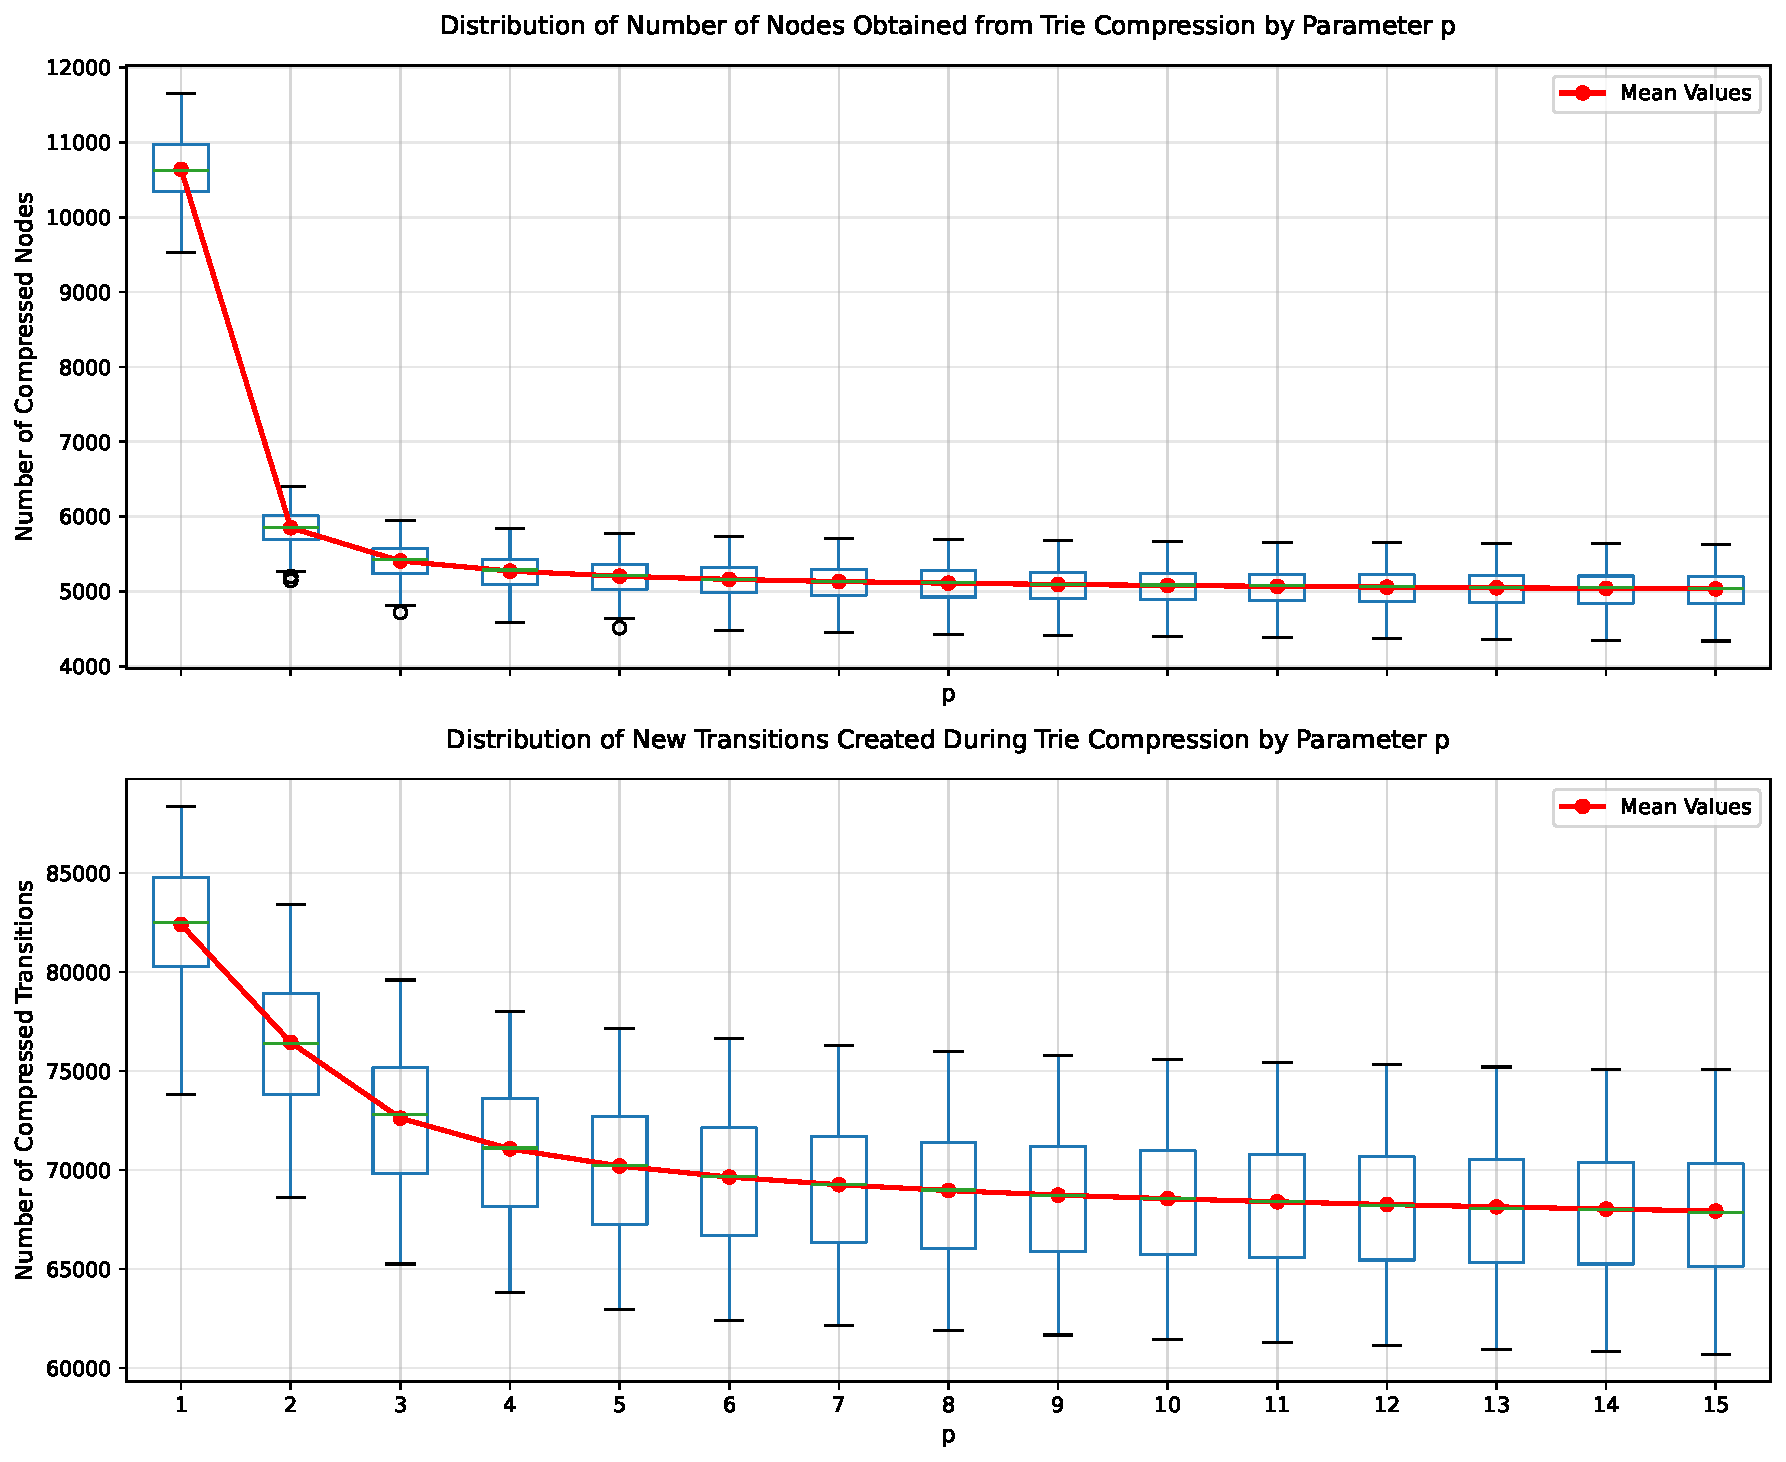
\includegraphics[width=1\linewidth]{Immagini/tree_compression_analysis_low.pdf}
    \caption{Experimental results for the \textbf{low-repetition} scenario. The plots show the number of nodes (top) and transitions (bottom) in the compressed automaton as a function of the co--lexicographical width, $p$. Each boxplot illustrates the distribution of results for a given $p$. The red line tracks the mean, showing a rapid decrease that approaches the theoretical minimum number of states (the mean number of MN--classes, shown by the green line).}
    \label{fig:exp_low_rep}
\end{figure}

\begin{figure}[H]
    \centering
    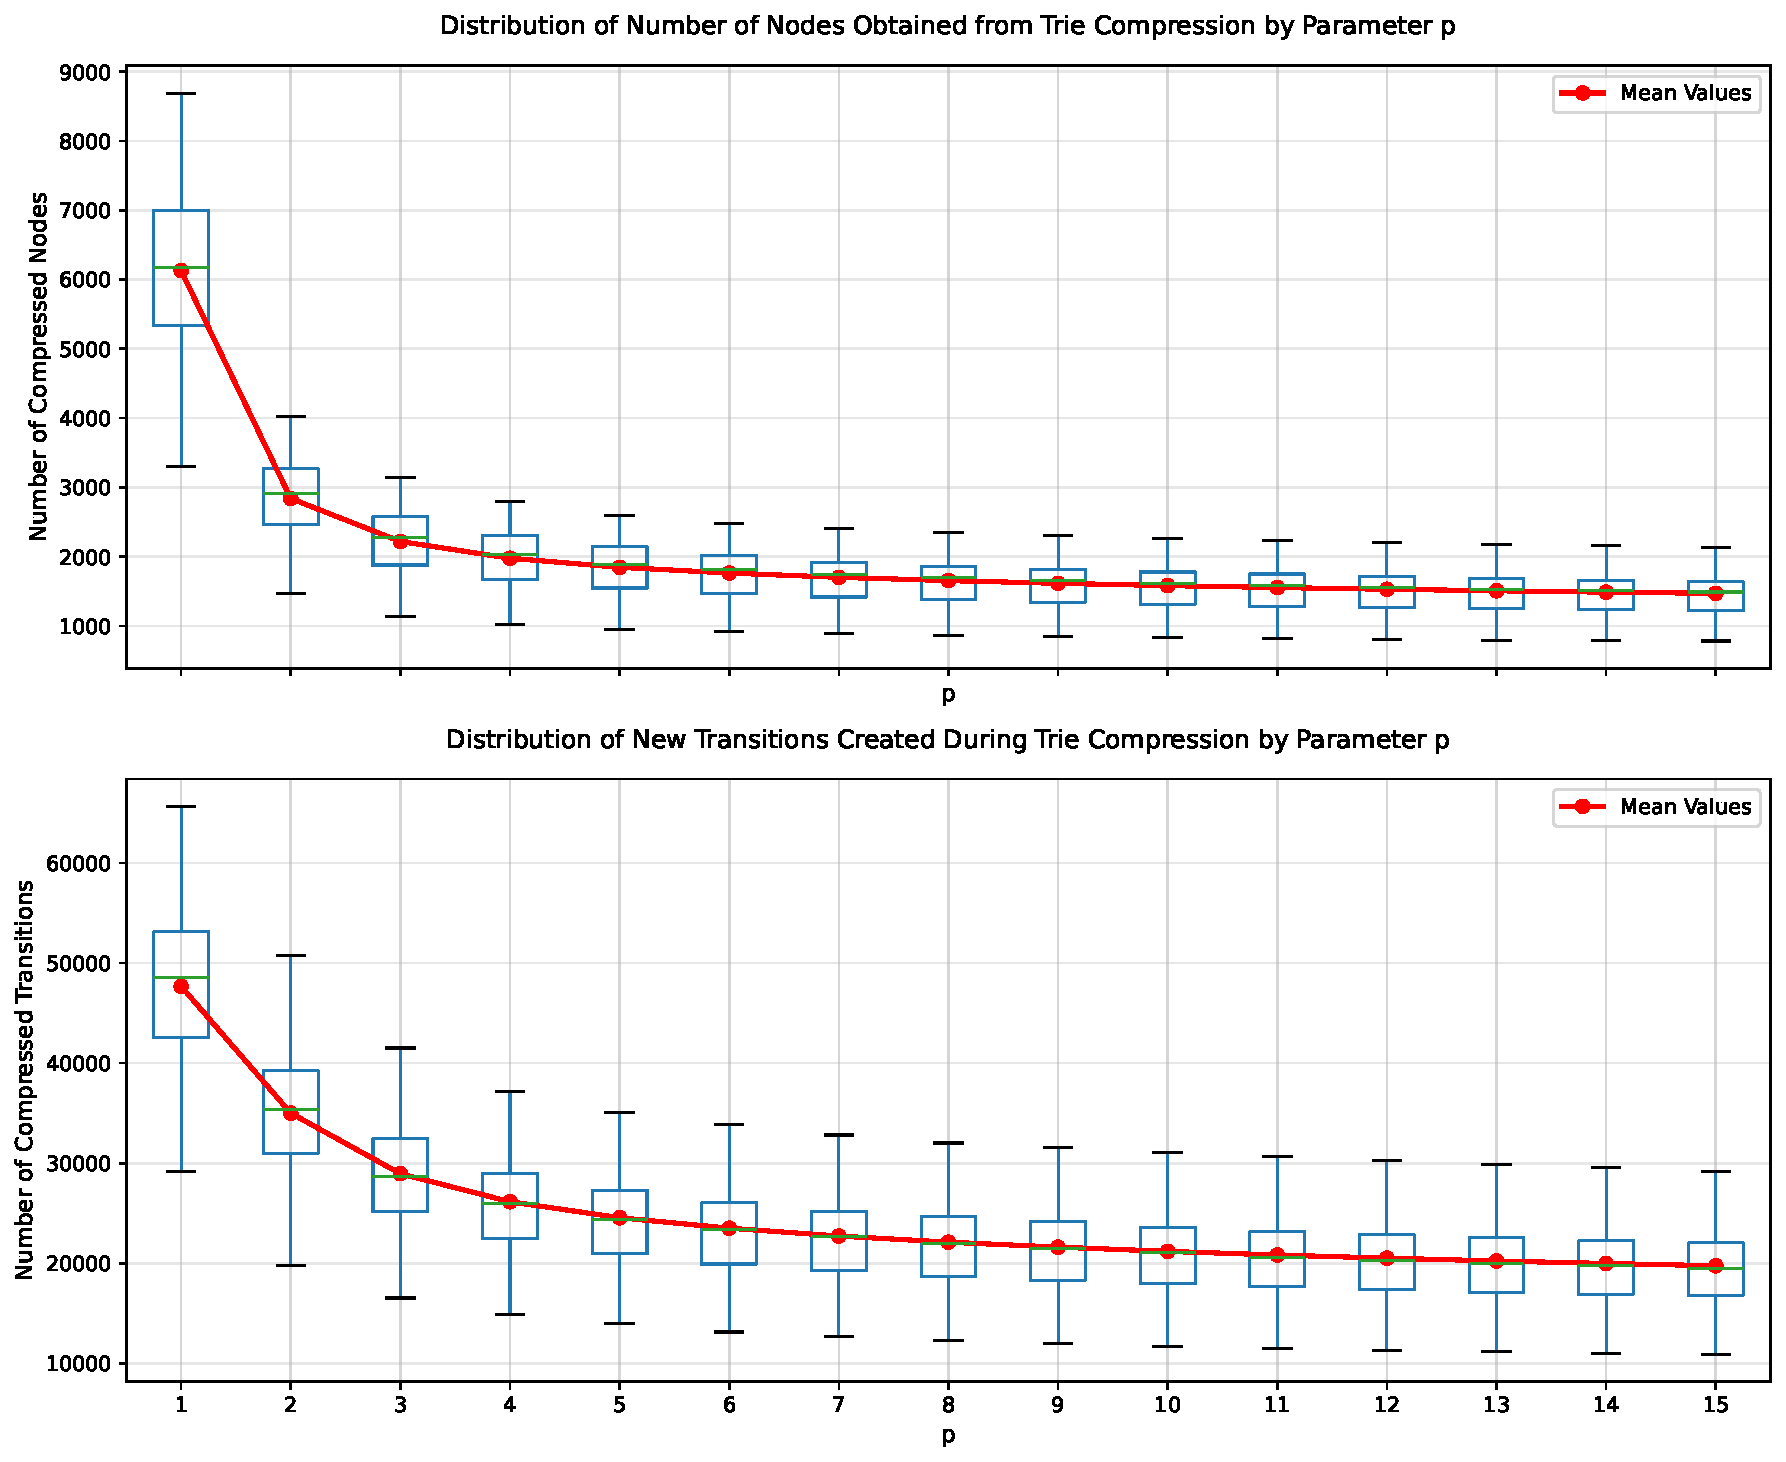
\includegraphics[width=1\linewidth]{Immagini/tree_compression_analysis_high.pdf}
    \caption{Experimental results for the highly-repetitive scenario. The plots show the number of nodes (top) and transitions (bottom) in the compressed automaton as a function of the co--lexicographical width, $p$. Each boxplot illustrates the distribution of results for a given $p$. The red line tracks the mean, showing a rapid decrease that approaches the theoretical minimum number of states (the mean number of MN--classes, shown by the green line).}
    \label{fig:exp_high_rep}
\end{figure}

To provide a clear comparison between the two scenarios, \cref{fig:exp_comparison} shows the mean and standard deviation for both the low- and high-repetitive datasets. The results confirm our hypothesis: tries with higher trie repetitiveness achieve significantly better compression, as evidenced by the lower number of nodes and transitions for all values of $p$. This is expected, as a more repetitive trie allow for a more compact representation in the compressed automaton.

\begin{figure}[H]
    \centering
    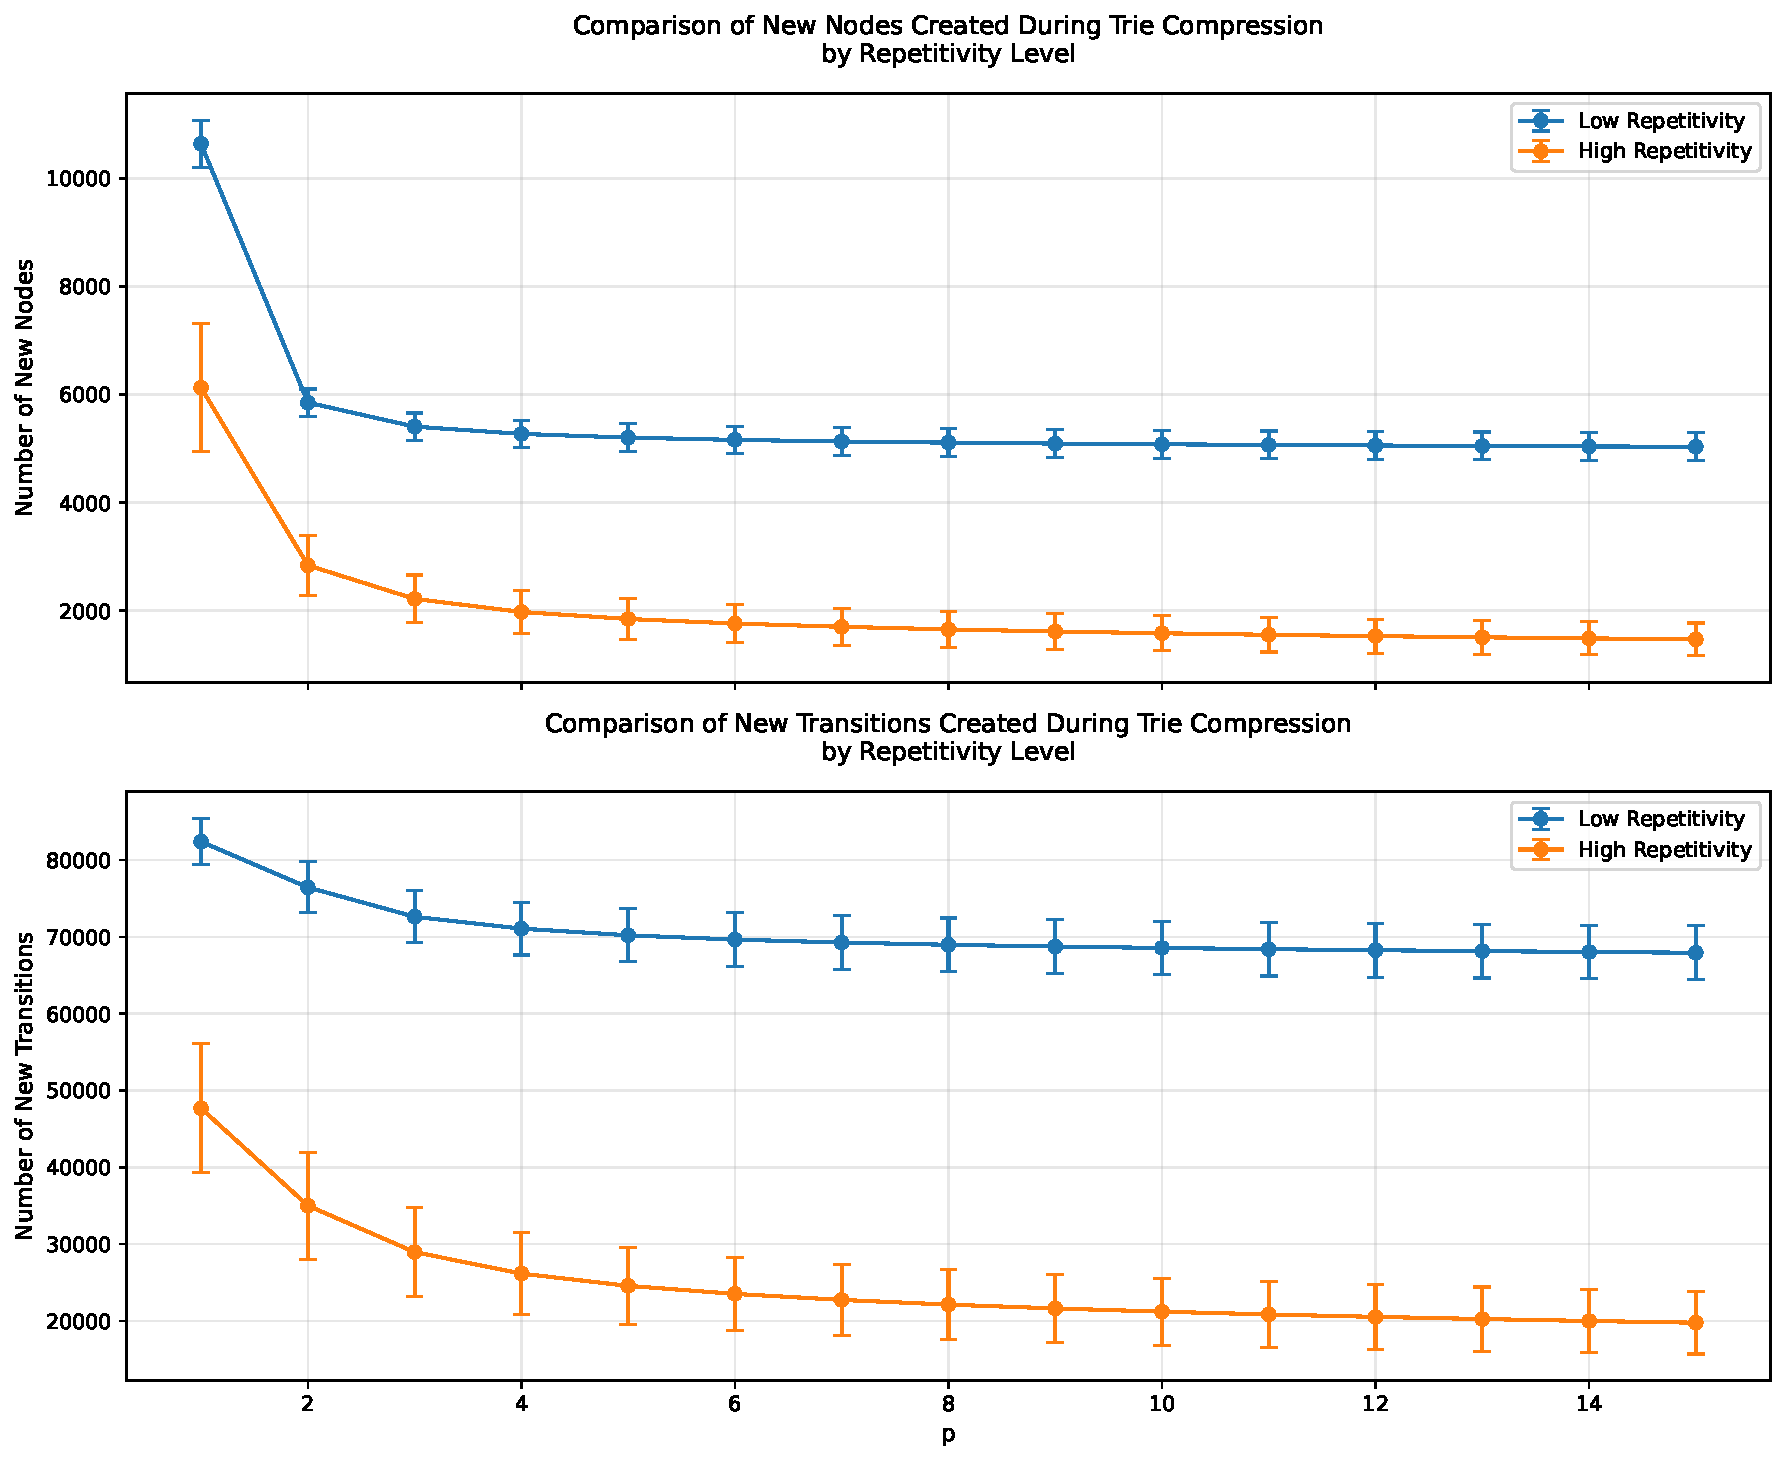
\includegraphics[width=1\linewidth]{Immagini/high_low_comparison.pdf}
    \caption{Direct comparison of compression performance for low-repetitive versus high-repetitive datasets. The plots track the mean number of nodes (top) and transitions (bottom) as a function of $p$. The results clearly show that high-repetitive datasets (orange) yield significantly better compression across all values of $p$, resulting in a much smaller final automaton. This highlights the effectiveness of our method in exploiting the redundancy present in highly repetitive data.}
    \label{fig:exp_comparison}
\end{figure}